   \documentclass [11pt]{article}
   \usepackage{latexsym}
   \usepackage{amssymb}
      \usepackage{amsmath}
      \usepackage{amsthm}
   \usepackage{url}
   \usepackage{tikz}

   \textwidth      15cm
   \textheight     23cm
   \oddsidemargin 0.5cm
   \topmargin    -0.5cm
   \evensidemargin\oddsidemargin


   \pagestyle{plain}




%
%  \newtheorem{theorem}{Theorem}
%  \newtheorem{lemma}[theorem]{Lemma}
%  \newtheorem{exercise}{Exercise}

  \newcommand{\ra}{\rightarrow}
  \newcommand{\Ra}{\Rightarrow}
  \newcommand{\La}{\Leftarrow}
  \newcommand{\la}{\leftarrow}
  \newcommand{\LR}{\Leftrightarrow}


\newcommand{\compl}[1]{\overline{#1}}

\renewcommand{\phi}{\varphi}
\renewcommand{\theta}{\vartheta}

\def\II{{\cal I}} 
\newcommand{\True}{\mathbf{true}}
\newcommand{\False}{\mathbf{false}}
\def\ox{\overline{x}} 
\def\oy{\overline{y}} 
\def\oz{\overline{z}} 



  \newcommand{\lto}{\rightarrow}
  \newcommand{\sto}{\Rightarrow}
  \newcommand{\snto}{\Leftarrow}
  \newcommand{\lnto}{\leftarrow}
  \newcommand{\siff}{\Leftrightarrow}
   \newcommand{\liff}{\leftrightarrow}
   \newcommand{\nmodels}{\not\models}

\newcommand{\clau}{\mathit{Clause}}
\newcommand{\var}{\mathit{Var}}
\newcommand{\lit}{\mathit{Lit}}
\newcommand{\dom}{\mathit{Dom}}

  \newtheorem{theorem}{Theorem}
  \newtheorem{lemma}[theorem]{Lemma}
  \newtheorem{corollary}[theorem]{Corollary}
    \newtheorem{observation}[theorem]{Observation}
  \newtheorem{proposition}[theorem]{Proposition}
  \newtheorem{conjecture}[theorem]{Conjecture}
  \newtheorem{definition}[theorem]{Definition}
  \newtheorem{example}[theorem]{Example}
  \newtheorem{remark}[theorem]{Remark}
  \newtheorem{exercise}[theorem]{Exercise}
 
 \newcommand{\reach}{\leadsto}
 \newcommand{\sreach}[1]{\stackrel{#1}{\leadsto}}

%%%%%%%%%%%%%%%%%%%%%%%%%%%%%%%%%%%%%%%%%%%%%%%%%%%%%%%%%%%%%%%%%%%

\begin{document}


%\maketitle



\medskip


\noindent
In the co-NL membership proof of {\bf 2-SAT}, the following reduction from {\bf co-2-SAT}
to the {\bf REACHABILITY} problem was given:

\begin{itemize}
\item The variables of $\phi$ and their negations form the vertices of
$G(\phi)$.
\item
There is an arc $(\alpha,\beta)$ iff there is a clause $\compl{\alpha}
\lor \beta$ or $\beta \lor \compl{\alpha}$ in $\phi$, 
where $\compl{\alpha}$ is the complement of $\alpha$, i.e.: If $\alpha$ is true
in some satisfying assignment ${\cal I}$ of $\phi$, then $\beta$ must also be true in ${\cal I}$.
\item It can be shown that $\phi$ is unsatisfiable iff there is a variable $x$ such that
there are paths from $x$ to $\neg x$ and from $\neg x$ to $x$ in
$G(\phi)$.
\end{itemize}

\noindent
{\em Notation.}
It is convenient to write $x \Ra y$ if $y$ is reachable from $x$ in 
the graph $G(\phi)$.

\begin{exercise}[4 credits]
{\em Give a rigorous proof of the 
``if''-direction of the correctness of the above reduction, i.e.: \\
%
If there exists a variable~$x$, s.t.\
$x \Ra  \neg x$ and $\neg x \Ra x$ in
$G(\phi)$, then $\phi$ is unsatisfiable.
}%em
\end{exercise}


\noindent
{\bf Hint.} Carefully distinguish between what is assumed, what is defined and what has to be shown. The proof could thus start as follows: 

\medskip
\noindent
{\bf Proof.} (indirect) 
Suppose that there exists a variable~$x$, s.t.\
$x \Ra  \neg x$ and $\neg x \Ra x$ in
$G(\phi)$. Moreover, suppose that there exists a model ${\cal I}$ of $\phi$. We derive a contradiction by showing that 
then both $x$ and $\neg x$ are true in ${\cal I}$. 


\paragraph*{Solution}


Before starting some notational conventions are to be established.

\begin{definition}
Let $G=\langle V,E \rangle$ be a graph. For two vertices $v,w \in V(G)$, let $v \sreach{G} w$ indicate that there exists a path from $v$ to $w$ in $G$. \footnote{$V(G)$ is the set of vertices, while $E(G)$ represents the set of edges of the given graph $G$.}
Moreover, if the graph in question is clear from the context, only $v \reach w$ shall be written.
\end{definition}



That is, rather than using the "$\sto$"-symbol, as suggested in the exercise description, the symbol  $ \leadsto $ is used. Thereby, avoiding a possible conflict with the semantic implication symbol entirely. 

\begin{remark}
Notice that the definition of the reachability problem, as presented in the slides, does not exclude paths of length $0$. Hence, it is trivially the case that $\forall x \in V(G) \; x \sreach{G} x$ for some graph $G$. 
\end{remark}

Moreover, to properly navigate propositional formulas consider the following.

\begin{definition}
\label{def:2cnf}
Let $\varphi=\bigwedge_{i=0}^n (l_{i} \lor l'_{i})$ be a propositional formula, with $l_i$ and $l'_i$ being literals and with $n\in \mathbb{N}$, i.e.\ $\varphi$ is a 2-CNF formula. Let $\var(\varphi)$ be the set of all atoms (boolean variables) in $\varphi$, let $\overline{\var}(\varphi):=\{\neg x \mid \forall x \in \var(\varphi)\}$ and let $\clau(\varphi)$ be the set of all clauses in $\varphi$.
%Alternatively, for $a,b \in \var(\varphi)$ let $E:= E_{11} \cup E_{10}\cup E_{01}\cup E_{00}$ with 
%\begin{itemize}
%\item $E_{11}:= \bigcup_{(a \lor b) \in \clau(\varphi)} \{ (\neg a, b), (\neg b, a) \}$
%\item $E_{10}:= \bigcup_{(a \lor \neg b) \in \clau(\varphi)} \{ (\neg a, \neg b), (b, a) \}$
%\item $E_{01}:= \bigcup_{(\neg a \lor  b) \in \clau(\varphi)} \{ (a,  b), (\neg b,\neg a) \}$
%\item $E_{00}:= \bigcup_{(\neg a \lor \neg b) \in \clau(\varphi)} \{ ( a, \neg b), ( b, \neg a) \}$
%\end{itemize}
\end{definition}

Furthermore, for the sake of completeness a restatement of the construction required during the reduction.


\begin{definition}
Consider the 2-CNF formula $\varphi$. Let $\mathcal{G}(\varphi):= \langle V,E \rangle$ where $V:= \var(\varphi) \cup \overline{\var}(\varphi)$ and $(a,b) \in E$ if and only if $\overline{a} \lor b \in \clau(\varphi)$ or  $b \lor \overline{a}  \in \clau(\varphi)$. 
%Alternatively, for $a,b \in \var(\varphi)$ let $E:= E_{11} \cup E_{10}\cup E_{01}\cup E_{00}$ with 
%\begin{itemize}
%\item $E_{11}:= \bigcup_{(a \lor b) \in \clau(\varphi)} \{ (\neg a, b), (\neg b, a) \}$
%\item $E_{10}:= \bigcup_{(a \lor \neg b) \in \clau(\varphi)} \{ (\neg a, \neg b), (b, a) \}$
%\item $E_{01}:= \bigcup_{(\neg a \lor  b) \in \clau(\varphi)} \{ (a,  b), (\neg b,\neg a) \}$
%\item $E_{00}:= \bigcup_{(\neg a \lor \neg b) \in \clau(\varphi)} \{ ( a, \neg b), ( b, \neg a) \}$
%\end{itemize}
\end{definition}
%
%
%Moreover, to remain congruent with Definition \ref{def:2cnf}, some satisfying assumptions are required.
%
%\begin{remark}
%W.l.o.g we can exclude all 2-CNF formulas of the form $\bigwedge_{i=0}^0 (l_{i} \lor l'_i)$ as empty 
%\end{remark}

Having defined all relevant concepts and having (hopefully) introduced all notational particularities. The next step is to establish some intermediary results. Initially, it has to be demonstrated that the edges in the constructed graph encode implications.


\begin{lemma}
\label{lemma:edge-implication}
For the 2-CNF formula $\varphi$, if $(a,b) \in E(\mathcal{G}(\varphi))$ then $\varphi \models a \to b$.
\end{lemma} 
\begin{proof}
Firstly, in the trivial case that $E(\mathcal{G}(\varphi))=\emptyset$, the implication holds vacuously.
Secondly, to verify the claim assume $(a,b) \in E(\mathcal{G}(\varphi))$. By construction, this implies that 
$\overline{a} \lor b \in \clau(\varphi)$ or  $b \lor \overline{a}\in \clau(\varphi)$, w.l.o.g (due to commutativity) assume it to be the prior. Thus, it follows that 
$\varphi \models \overline{a} \lor b$. However, since $\overline{a}$ is logical equivalent to $\neg a$, i.e. if $a = p$ then $\overline{a} = \neg p$ and if $a = \neg p$ then $\overline{a} =  p$, one obtains $\varphi \models \neg a \lor b$. Finally, from the definition of implication one can finally conclude that $\varphi \models a \to b$.
\end{proof}


This single result suffices to show the main result of this exercise. Hereby, the suggested start, as presented in the exercise description, shall serve as the beginning of the proof for the following lemma.


\begin{lemma}
For the 2-CNF formula $\varphi$, if there exists $x \in \var(\varphi)$ such that $x \sreach{\mathcal{G}(\varphi)} \neg x$ and $\neg x \sreach{\mathcal{G}(\varphi)} x$,  then $\varphi$ is unsatisfiable. That is,
\begin{equation*}
 \exists x \in \var(\varphi)\;  x \sreach{\mathcal{G}(\varphi)} \neg x \land \neg x \sreach{\mathcal{G}(\varphi)} x \implies \nmodels \varphi 
\end{equation*}
\end{lemma} 
\begin{proof}
Suppose that there exists a variable~$x$, s.t.\
$x \reach  \neg x$ and $\neg x \reach x$ in
$\mathcal{G}(\phi)$. Moreover, suppose that there exists a model ${\cal I}$ of $\phi$. We derive a contradiction by showing that 
then both $x$ and $\neg x$ are true in ${\cal I}$. 

Starting with $x \reach  \neg x$. By definition of reachability one obtains that there exists a sequence $S=(s_i)_{i\in I}$ of edges, i.e. $\forall i \in I \; s_i\in E(\mathcal{G}(\varphi))$, where 
$I :=\{0 , \dots,n\}$ for $0 < n \leq  |E(\mathcal{G}(\varphi))| $ such that $s_0=(x,l_1)$ and $s_n=(l_n,\neg x)$.
As Lemma \ref{lemma:edge-implication} established, for an arbitrary $s_i=(l_i,l_{i+1})$ it follows that $\varphi \models l_i \lto l_{i+1}$.
That is, from the sequence $S$ one obtains that 
\begin{equation*}
\varphi \models (x\lto l_{1}) \land \dots \land  (l_n \lto \neg x)
\end{equation*}
Now by iteratively applying the propositional tautology $((p \to q) \land (q \to r)) \to (p \to r)$ one obtains $\varphi \models x \lto \neg x$.\footnote{
For the sake of completion a single step is demonstrated. Starting from 
$\varphi \models (x\lto l_{1}) \land  (l_{1} \lto l_2) \land \dots \land  (l_n \lto \neg x)$ using $\varphi \models \big((x\lto l_{1}) \land  (l_{1} \lto l_2)\big) \to  (x\lto l_2)$
it follows by weakening and semantics of conjunction that  $\varphi \models   (x \lto l_2) \land \dots \land  (l_n \lto \neg x)$.
To be formally correct, one ought to demonstrate this claim by induction. However, since the transitivity of implication is a well known fact in classical logic, this unnecessary labour will be spared. 
%
%
%$\varphi \models \big((x\lto l_{1}) \land  (l_{1} \lto l_2) \dots \land  (l_n \lto \neg x) \big)\to \big( (l_x \lto l_2) \dots \land  (l_n \lto \neg x)\big)$ and thus one obtains  $\varphi \models   (l_x \lto l_2) \dots \land  (l_n \lto \neg x)$ 
} 

The same argument in analogue holds for $\neg x \reach x$. 
Hence, one obtains $\varphi \models  (x \lto \neg x) \land (\neg x \lto  x) $. Now given the assumption that there exists an interpretation $\mathcal{I}$ such that $\mathcal{I} \models \varphi$ it must be by definition that $\mathcal{I} \models  (x \lto \neg x) \land (\neg x \lto  x) $, which clearly is impossible. That is, if $\mathcal{I}\models x$ then it must be that  $\mathcal{I}\models \neg x$ by $(x \lto \neg x)$ which by semantics is impossible, and if  $\mathcal{I}\nmodels x$ by semantics $\mathcal{I}\models \neg x$ and thus by $(\neg x \lto  x)$ it must be that $\mathcal{I}\models x$, which again is impossible. Therefore, $\mathcal{I}$ can not exists, thus verifying the claim. 


\end{proof}


\newpage
\bigskip


\noindent
For the ``only if''-direction of the correctness proof of the 
problem reduction from {\bf co-2-SAT}
to {\bf REACHABILITY}, we have to show the following implication: If there exists no 
variable~$x$, s.t.\
$x \Ra  \neg x$ and $\neg x \Ra x$ in
$G(\phi)$, then there 
exists a model $\II$ of $\phi$.
To this end, consider the truth assignment $\II$ constructed by the following algorithm: 
%
%
\begin{tabbing}
123\=123\=123\=123\=123\=123\=\kill
/* Step 1 */  \\
{\bf for each} literal $x$, s.t.\ $\overline{x} \Ra x$ 
{\bf do} \\
\> $\II(x) := \True$;
 /* hence, implicitly, $\II(\ox) := \False$; */ \\
\> {\bf for each} literal $z$ with $x \Ra z$ 
{\bf do}  $\II(z) := \True$ {\bf od};
\\
{\bf od}; 
\\[1.1ex]
/* Step 2 */  \\
{\bf while} there exists $x \in Var(\phi)$, s.t.\ $\II(x)$ is undefined
{\bf do} \\
\> choose an arbitrary variable $x$, s.t.\ $\II(x)$ is undefined; \\
\> $\II(x) := \True$;  \\
\> {\bf for each} literal $z$ with $x \Ra z$ 
{\bf do}  $\II(z) := \True$ {\bf od};\\
{\bf od};
\end{tabbing}
%
%
To show that an assignment $\II$ thus constructed is indeed a 
model of $\phi$, it is convenient to proof the following lemmas.

\begin{lemma}
\label{lem:1}
Suppose that there exists no
variable $x$, s.t.\ both $x \Ra \ox$ and $\ox \Ra x$ hold.
Then a truth assigment made by the above algorithm is never changed later, i.e.: it cannot happen, that at some stage, 
$\II (z) =\True$ for some variable $z$ and later this value is changed to 
$\II (z) =\False$ or vice versa.
\end{lemma}



\begin{lemma}
\label{lem:2}
Suppose that there exists no
variable $x$, s.t.\ both $x \Ra \ox$ and $\ox \Ra x$ hold.
Then the truth assigment $\II$ constructed by the above algorithm
is a model of $\phi$.
\end{lemma}

\smallskip

\newpage

\noindent
\begin{exercise}[4 credits]
{\em Give a rigorous proof of Lemma \ref{lem:1}.
}%em
\end{exercise}

\noindent
\paragraph*{Solution}

Firstly, some auxiliary results.

\begin{lemma}
\label{lem:inverse-path}
Let $\varphi$ a 2-CNF formula. If for two literals $x$ and $y$ in $\varphi$, it holds that $x\sreach{\mathcal{G}(\varphi)} y $ then it must be that $\overline{y} \sreach{\mathcal{G}(\varphi)} \overline{x}$.
\end{lemma}
\begin{proof}
This can be shown by induction on the length of the path between $x$ and $y$.
\begin{itemize}
\item \textbf{IH:} If there exists a path of length $n$ in $\mathcal{G}(\varphi)$ starting at $x$ and ending at $y$, then there exists a path starting $\overline{y}$ and ending at $\overline{x}$.
\item \textbf{IB:} If the path is of length $0$ and one has $x \reach y$ then it must be the case that $y = x$, i.e. $x \reach x$. 
Hence, $\overline{x} \reach \overline{x}$ ought to be established. However, this claim is already validated through the definition of reachability.
%then $(x,y) \in \mathcal{G}(\varphi)$, which implies that there exists $\overline{x} \lor y$ or $y\lor \overline{x} $ as clause in $\varphi$. W.l.o.g. assume it to be the prior.
%By construction,  $(a,b) \in E(\mathcal{G}(\varphi))$ if and only if $\overline{a} \lor b \in \clau(\varphi)$ or  $b \lor \overline{a}  \in \clau(\varphi)$. Hence, the clause  $\overline{x} \lor y$ initially read as $\overline{a} \lor b$ could also be read as $b \lor \overline{a}$. 
%Hence, $(a,b)=(\overline{y},\overline{x}) \in E(\mathcal{G}(\varphi))$
\item \textbf{IH:} Assume there exists a path of length $n+1$ from $x$ to $y$. Hence, there exists an $z \in V(\mathcal{G}(\varphi))$ such that $x \reach z$ through a path of length $n$ and $(z,y) \in E(\mathcal{G}(\varphi))$. By \textbf{IH}, $\overline{z} \reach \overline{x}$. It is known that $(\alpha, \beta) \in E(\mathcal{G}(\varphi))$ if and only if $\overline{\alpha} \lor  \beta \in \clau(\varphi)$ or  $\beta \lor \overline{\alpha}  \in \clau(\varphi)$.
Therefore, from $(z,y) \in E(\mathcal{G}(\varphi))$ it follows by construction that either $\overline{z} \lor y \in \clau(\varphi)$ or $y \lor \overline{z}  \in \clau(\varphi)$. In the prior, consider $\alpha=\overline{y}$ and $\beta = \overline{z}$, thus $\overline{z} \lor y= \beta \lor \overline{\alpha}$ and therefore $(\alpha, \beta)= (\overline{y}, \overline{z}) \in E(\mathcal{G}(\varphi))$. And in the latter, consider $\alpha=\overline{y}$ and $\beta = \overline{z}$, thus $y \lor \overline{z}= \overline{\alpha} \lor \beta$ and therefore $(\alpha, \beta)= (\overline{y}, \overline{z}) \in E(\mathcal{G}(\varphi))$. Or put simply, by construction of $\mathcal{G}(\varphi)$, it must be that if $(x,y) \in E(\mathcal{G}(\varphi))$ then $(\overline{y}, \overline{x}) \in E(\mathcal{G}(\varphi))$. Finally, permitting the conclusion $\overline{y} \sreach{\mathcal{G}(\varphi)} \overline{x}$.
\end{itemize}
\end{proof}

%
%Secondly, a slight reformulation of the given algorithm.
%
%\begin{definition}
%Let $\varphi$ a 2-CNF formula. Consider the following algorithm $\mathcal{A}_1$ taking $\varphi$ as input.
%
%
%\begin{tabbing}
%123\=123\=123\=123\=123\=123\=\kill
%$\mathcal{A}_1(\varphi)$:\\
%\> $n := 0$;\\
%\> {\bf for each} $x \in \lit(\varphi)$ , s.t.\ $\overline{x} \sreach{\mathcal{G}(\varphi)} x$  {\bf do}    \\
%\> \> $n := n+1$;\\
%\> \> $\mathcal{J}_n(x) := \True$; \\
%\> \> {\bf for each} $z \in \lit(\varphi)$ with $x  \sreach{\mathcal{G}(\varphi)} z$ {\bf do} \\
%\> \>\> $\mathcal{J}_n(z) := \True$; \\
%\> \>{\bf od};\\
%\> {\bf od}; 
%\> {\bf return} $\mathcal{J}_n$;
%\end{tabbing}
%
%Furthermore, consider $\mathcal{A}_2$ taking $\varphi$ and a possibly partial interpretation $\mathcal{J}$ as input
%
%\begin{tabbing}
%123\=123\=123\=123\=123\=123\=\kill
%$\mathcal{A}_2(\mathcal{J},\varphi)$:\\
%\> $n := 0$;\\
%\> $\mathcal{J}_n:= \mathcal{J}$; \\
%\> {\bf while}  $\exists x \in\var(\phi)$, s.t.\ $x \notin \dom(\mathcal{J})$ {\bf do}  \\
%\> $n := n+1$;\\
%\>\>  choose an arbitrary $x \in \var(\varphi)$, s.t.\ $\mathcal{J}(x)=\{\}$;\\
%\>\>  $\mathcal{J}_n(x) := \True$;  \\
%\>\>  {\bf for each} $z\in \lit(\varphi)$ with $x  \sreach{\mathcal{G}(\varphi)} z$   {\bf do} \\
%\> \>\> $\mathcal{J}_n(z) :=\True$; \\
%\> \>{\bf od};\\
%\> {\bf od};\\
%\> {\bf return} $\mathcal{J}_n$;
%\end{tabbing}
%
%Using those two algorithms let $\mathcal{A}(\varphi):= \mathcal{A}_2\big(\mathcal{A}_1(\varphi),\varphi\big)$.
%\end{definition}
%
%
%
%Moreover, as a partial solution consider the following Lemma.
%
%\begin{lemma}
%\label{lem:1-step1}
%Let $\varphi$ a 2-CNF formula. Consider  $\mathcal{J}_n :=\mathcal{A}_1$. Suppose that there exists no variable $x \in \var(\varphi)$, s.t.\ both $x \sreach{\mathcal{G}(\varphi)} \ox$ and $\ox \sreach{\mathcal{G}(\varphi)}  x$ hold. 
%Then for some $0 \leq k <n$ it holds that $\forall x\in \var(\varphi)\; x \in \dom(\mathcal{J}) \sto \mathcal{J}_k(x) = \mathcal{J}_{k+1}(x)$.
%\end{lemma}

\begin{remark}
What follows is the unfortunate result of inertia. That is, the approach presented above, initially perceived to be more elegant, merely resulted in additional overhead.
However, time constraints barred a sensible reformulation of this proof in a more direct fashion. Hence, my dearest apologies to the reader for the additional work.
\end{remark}

Secondly, to reduce some of the procedural aspects a slight modification of the given algorithm.

\begin{definition}
Let $\varphi$ a 2-CNF formula. Then let $\mathcal{J}$ be computed using the following algorithm $\mathcal{A}$


\begin{tabbing}
123\=123\=123\=123\=123\=123\=\kill
/* Step 0 */ \\
\> {\bf for each} $x \in \var(\varphi)$ {\bf do}  $\mathcal{J}(z) :=\{\}$ {\bf od};\\
/* Step 1 */  \\
{\bf for each} $x \in \lit(\varphi)$ , s.t.\ $\overline{x} \sreach{\mathcal{G}(\varphi)} x$  {\bf do}   /*Loop A*/ \\
\> $\mathcal{J}(x) := \mathcal{J}(x) \cup \{ \True\}$; \\
\> $\mathcal{J}(\ox) := \mathcal{J}(\ox) \cup \{ \False\}$; \\
\> $\mathcal{I}(x) := \True$; \\
\> {\bf for each} $z \in \lit(\varphi)$ with $x  \sreach{\mathcal{G}(\varphi)} z$ {\bf do} \\
\>\> $\mathcal{J}(z) := \mathcal{J}(z) \cup \{ \True\}$; \\
\>\> $\mathcal{J}(\overline{z}) := \mathcal{J}(\overline{z}) \cup \{ \False\}$; \\
\>\> $\mathcal{I}(z) := \True$; \\
\>{\bf od};\\
{\bf od}; 
\\[1.1ex]
/* Step 2 */  \\
{\bf while}  there exists $x \in \var(\phi)$, s.t.\ $\II(x)$ is undefined {\bf do}  /*Loop B*/  \\
%$\exists x \in\var(\phi)$, s.t.\ $\mathcal{J}(x)=\{\}$ {\bf do}  /*Loop B*/ \\
\> choose an arbitrary $x \in \var(\varphi)$, s.t.\ $\mathcal{J}(x)=\{\}$;\\
\> $\mathcal{J}(x) := \mathcal{J}(x) \cup \{ \True\}$;  \\
\> $\mathcal{J}(\overline{x}) := \mathcal{J}(\overline{x}) \cup \{ \False\}$; \\
\> $\mathcal{I}(x) := \True$; \\
\> {\bf for each} $z\in \lit(\varphi)$ with $x  \sreach{\mathcal{G}(\varphi)} z$   {\bf do} \\
\>\> $\mathcal{J}(z) := \mathcal{J}(z) \cup \{ \True\}$; \\
\>\> $\mathcal{J}(\overline{z}) := \mathcal{J}(\overline{z}) \cup \{ \False\}$; \\
\>\> $\mathcal{I}(z) := \True$; \\
\>{\bf od};\\
{\bf od};\\
{\bf return} $\mathcal{J}$;
\end{tabbing}
\end{definition}

That is, the algorithm defined above differs only from the original one, in the fact that parallel to the construction of $\mathcal{I}$ another object is constructed. Namely, $\mathcal{J}$ which mirrors $\mathcal{I}$, but for the fact that rather than re-assigning truth values it simply adds them.  Moreover, it is clear to see that the \texttt{while}-condition $\exists x \in \var(\phi) \; \II(x) \textit{ is undefined}$ is equal to the condition $\exists x \in\var(\phi) \; \mathcal{J}(x)=\{\}$. 
To proof Lemma \ref{lem:1-alt}, which is a slight reformulation of Lemma \ref{lem:1}, consider the following results.




%
%\begin{lemma}
%\label{lem:1-alt-loop}
%Let $\varphi$ a 2-CNF formula. Let $\mathcal{J}= \mathcal{A}(\varphi)$ For a literal $x$, if $\overline{x} \sreach{\mathcal{G}(\varphi)} x$ and if $\False \in \mathcal{J}(\overline{x})$, $\True \in \mathcal{J}(x)$ and if there exists a literal $y$ in $\varphi$ such that $x \sreach{\mathcal{G}(\varphi)} y$, then $x \sreach{\mathcal{G}(\varphi)} \overline{x}$.
%\end{lemma}
%\begin{proof}
%Assume that this is the case. That is, one has a literal $x$ from $\varphi$ where $\overline{x} \sreach{\mathcal{G}(\varphi)} x$, such that $\False \in \mathcal{J}(\overline{x})$ and $\True \in \mathcal{J}(x)$. Moreover, there exists literal $y$ in $\varphi$ such that $x \sreach{\mathcal{G}(\varphi)} y$. Thereby, it follows from $\overline{x} \reach  x$ and $x\reach y$ that $\overline{x} \reach  y$. From Lemma \ref{lem:inverse-path} it follows that $\overline{y} \reach x$ as well as $\overline{y} \reach \overline{x}$.d
%\end{proof}

%\begin{lemma}
%\label{lem:1-alt-step1}
%Let $\varphi$ a 2-CNF formula. Suppose that there exists no variable $x \in \var(\varphi)$, s.t.\ both $x \sreach{\mathcal{G}(\varphi)} \ox$ and $\ox \sreach{\mathcal{G}(\varphi)}  x$ hold.
%Let  $\mathcal{J}$ be the function constructed by \texttt{Step 1} of $\mathcal{A}(\varphi)$. Then it holds that for all literals $x$ in $\varphi$
%if $\True \in \mathcal{J}(x)$, then there exists a literal $z$ such that $\overline{z} \reach z$ and $z \reach x$.
%\end{lemma}


\begin{lemma}
\label{lem:1-alt-step1}
Let $\varphi$ a 2-CNF formula. Suppose that there exists no variable $x \in \var(\varphi)$, s.t.\ both $x \sreach{\mathcal{G}(\varphi)} \ox$ and $\ox \sreach{\mathcal{G}(\varphi)}  x$ hold.
Let  $\mathcal{J}$ be the function constructed by \texttt{Step 1} of $\mathcal{A}(\varphi)$. Then it holds that for all literals $x$ in $\varphi$, $|\mathcal{J}(x)|\leq 1$ and $\mathcal{J}(x) \cap \mathcal{J}(\overline{x}) = \emptyset$ and $|\mathcal{J}(x)| = |\mathcal{J}(\overline{x})|$.
\end{lemma}
\begin{proof}
This result shall be demonstrated by means of induction. That is, under the assumption that $|\mathcal{J}(x)|\leq 1$ and $\mathcal{J}(x) \cap \mathcal{J}(\overline{x}) = \emptyset$ and $|\mathcal{J}(x) |= |\mathcal{J}(\overline{x})|$ after $n$  iterations of \texttt{Loop A}, it will be established that $|\mathcal{J}(x)|\leq 1$ and $\mathcal{J}(x) \cap \mathcal{J}(\overline{x}) = \emptyset$ and $|\mathcal{J}(x)| = |\mathcal{J}(\overline{x})|$ hold after $n+1$ iterations.
\begin{itemize}
\item \textbf{IH:} After $n$ iterations of \texttt{Loop A}, it holds that for all literals $x$ in $\varphi$, $|\mathcal{J}(x)|\leq 1$ and $\mathcal{J}(x) \cap \mathcal{J}(\overline{x}) = \emptyset$ and $|\mathcal{J}(x)| = |\mathcal{J}(\overline{x})|$.
\item \textbf{IB:} Clearly, for the $0^{\text{th}}$ iteration the statement holds trivially.
%Before the first iteration $\forall l \in \mathit{Lit}(\varphi)\; \mathcal{J}(l)=\emptyset$. Assume that $x \in \lit(\varphi)$ was chosen. Hence, $\overline{x} \reach x\;^{(0)}$.Towards a contradiction, assume that after the first iteration, there exists a literal $y$ such that $|\mathcal{J}(y)|=2$. $\True \in \mathcal{J}(y)$ forces $x\reach y\;^{(1)}$ by construction . That is, starting with all assignments being empty sets the algorithm only assigning $\True$ to some literal $z$ (including $x$) if $x\reach z$. However, for $\False \in \mathcal{J}(y)$ it must be that $\True \in \mathcal{J}(\overline{y})$ was added. However, this would imply that  $x\reach \overline{y}\;^{(1)}$. Now by Lemma \ref{lem:inverse-path} it follows from $x\reach \overline{y}$ that $ y\reach \overline{x}\;^{(1)}$. Using this and the fact that $x\reach y$ a loop is obtained, i.e. $x\reach \overline{x}$ was established. That is,
%
%\begin{center}
%\begin{tikzpicture}
%  \tikzset{vertex/.style = {draw=none,minimum size=1.5em,inner sep=0.5pt}}
%  \tikzset{edge/.style = {-,-> = latex', dashed}}
%  
%  
%\node[vertex] (ox)  at (0,0.5) {$\overline{x}$};
%\node[vertex] (x)  at (2,0.5) {$x$};
%\node[vertex] (y)  at (4,0) {$y$};
%\node[vertex] (oy)  at (4,1) {$\overline{y}$};
%
%  
%    \path[->](ox) edge[dotted, thick] node [above]{\tiny(0)} (x);
%      \path[->](x) edge[dotted, thick] node [above]{\tiny(1)} (y);
%        \path[->](x) edge[dotted, thick] node [above]{\tiny(2)} (oy);
%   
%    \path[->](y) edge[dotted,bend left=20, thick] node [below]{\tiny(3)} (ox);
%\end{tikzpicture}
%\end{center}
%Hence, $\forall x \in \mathit{Lit}(\varphi)\; |\mathcal{J}(x)|\leq 1$. Finally, as the algorithm always adds the complementary values to complementary literals the second statement, $\forall x \in \mathit{Lit}(\varphi)\;  \mathcal{J}(x) \cap \mathcal{J}(\overline{x}) = \emptyset$, follows immediately.

\item \textbf{IS:} By \textbf{IH}  $\forall x \in \mathit{Lit}(\varphi)\; |\mathcal{J}(x)|\leq 1 \land \mathcal{J}(x) \cap \mathcal{J}(\overline{x}) = \emptyset \land |\mathcal{J}(x)| = |\mathcal{J}(\overline{x})|$,
before the execution of the $n+1$ iteration. Assume that the literal $x$ was chosen. Hence, it is known that $\overline{x} \reach x\;^{(0)}$. Towards a contradiction assume that there exists a literal $y$ such that $|\mathcal{J}(y)|=2$ after the $n+1^{\text{th}}$ execution of \texttt{Loop A}.\footnote{Before diving into the subsequent case distinction, notice that $y$ could be $x$ or $\overline{x}$. Moreover, it is unnecessary to cover both of those possibilities, as (by construction) one can not exists without the other.  That is, if $y=\overline{x}$ and $|\mathcal{J}(y)|=2$ after the  $n+1^{\text{th}}$ iteration, it must be by definition of $\mathcal{A}$ that  $|\mathcal{J}(x)|=2$ as well, thus allowing one to show this claim for $x$ only. However, the cases are constructed such that they include those cases without explicitly engaging with them (see the \emph{Appendix }for a demonstration of this claim)}
Hence, there are three cases. 
\begin{itemize}
\item $\mathcal{J}(y)=\{\}$ before the $n+1^{\text{th}}$ iteration of \texttt{Loop A}. Hence, it must be that $\True$ and $\False$  were added during the $n+1^{\text{th}}$ iteration of \texttt{Loop A}. This implies, by construction, that $x \reach y\; ^{(1)}$ and $x \reach \overline{y}\; ^{(2)}$, as this is the only manner in which $\True$ could have been added to both during \texttt{Loop A}. Using Lemma \ref{lem:inverse-path}, this implies that $y \reach \overline{x}\;^{(3)}$ and $\overline{y} \reach \overline{x}\;^{(4)}$. However, either is sufficient to establish that $x \reach \overline{x}$. Thereby, creating a cycle and subsequently a contradiction. 

\begin{center}
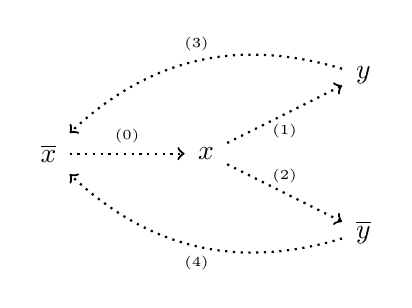
\begin{tikzpicture}
  \tikzset{vertex/.style = {draw=none,minimum size=1.5em,inner sep=0.5pt}}
  \tikzset{edge/.style = {-,-> = latex', dashed}}
  
  
\node[vertex] (ox)  at (0,1) {$\overline{x}$};
\node[vertex] (x)  at (2,1) {$x$};
\node[vertex] (y)  at (4,2) {$y$};
\node[vertex] (oy)  at (4,0) {$\overline{y}$};


  
    \path[->](ox) edge[dotted, thick] node [above]{\tiny(0)} (x);
      \path[->](x) edge[dotted, thick] node [below]{\tiny(1)} (y);
            \path[->](x) edge[dotted, thick, ] node [above]{\tiny(2)} (oy);
          
        
        \path[->](y) edge[dotted, thick, bend right=30] node [above]{\tiny(3)} (ox);
        \path[->](oy) edge[dotted, thick, bend left=30] node [below]{\tiny(4)} (ox);
   

\end{tikzpicture}
\end{center}
 
 
 
\item $\mathcal{J}(y)=\{\False\}$ before the $n+1^{\text{th}}$ iteration of \texttt{Loop A}. Therefore, $\True$ must have been added. Hence, it must be that $x \reach y\;^{(1)}$, as otherwise $\True$ would not have been added in the $n+1^{\text{th}}$ iteration of \texttt{Loop A}. Moreover, by \textbf{IH} it must be that $\mathcal{J}(\overline{y})=\{\True\}$ before the $n+1^{\text{th}}$ iteration of \texttt{Loop A}. This implies, by definition of \texttt{Loop A}, that there must exist a $z \in \lit(\varphi)$  (possibly $\overline{y}$ itself) such that 
$\overline{z} \reach z\; ^{(2)}$ and $z \reach \overline{y}\; ^{(3)}$. As this is the only way for $\overline{y}$ to obtain the truth value $\True$ during \texttt{Loop A}. Now, from $z \reach \overline{y}$ one obtains $y \reach \overline{z}\;^{(4)}$ 
through Lemma \ref{lem:inverse-path}. Similarly, one obtains from $x \reach y$ that $\overline{y} \reach \overline{x}\;^{(5)}$. Thereby, creating a cycle and thus a contradiction.

\begin{center}
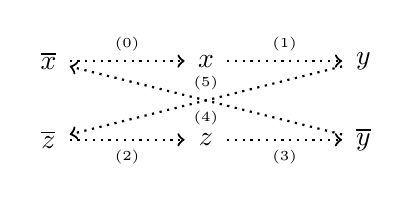
\begin{tikzpicture}
  \tikzset{vertex/.style = {draw=none,minimum size=1.5em,inner sep=0.5pt}}
  \tikzset{edge/.style = {-,-> = latex', dashed}}
  
  
\node[vertex] (ox)  at (0,1) {$\overline{x}$};
\node[vertex] (x)  at (2,1) {$x$};
\node[vertex] (y)  at (4,1) {$y$};
\node[vertex] (oy)  at (4,0) {$\overline{y}$};
\node[vertex] (z)  at (2,0) {$z$};
\node[vertex] (oz)  at (0,0) {$\overline{z}$};

  
    \path[->](ox) edge[dotted, thick] node [above]{\tiny(0)} (x);
      \path[->](x) edge[dotted, thick] node [above]{\tiny(1)} (y);
      
        \path[->](oz) edge[dotted, thick] node [below]{\tiny(2)} (z);
        \path[->](z) edge[dotted, thick] node [below]{\tiny(3)} (oy);
        
        \path[->](y) edge[dotted, thick] node [above]{\tiny(5)} (oz);
        \path[->](oy) edge[dotted, thick] node [below]{\tiny(4)} (ox);
   

\end{tikzpicture}
\end{center}
 

\item $\mathcal{J}(y)=\{\True\}$ before the $n+1^{\text{th}}$ iteration of \texttt{Loop A}. Thus, by \textbf{IH} it must be that $\mathcal{J}(\overline{y})=\{\False\}$ before the said iteration. If $\False$ was added to $\mathcal{J}(y)$ at the $n+1^{\text{th}}$ iteration, then by construction it must be that $\True$ was added to $\mathcal{J}(\overline{y})$ at the same time. However, for $\True$ to be added to a literal at step $n+1$ if must be that it is reachable from $x$. Hence, one obtains that $x \reach \overline{y}\;^{(1)}$. 
%As a side note, observe that this covers the case where $y=\overline{x}$ and that the case $y=x$ is an impossibility.
Now the argument is an analogue to the previous case. That is, as $\mathcal{J}(y)=\{\True\}$ after iteration $n$. Again by definition of \texttt{Loop A}  it must be the case that there exist a $z\in \lit(\varphi)$ such that $\overline{z} \reach z\;^{(2)}$ and $z \reach y\;^{(3)}$. Now through Lemma \ref{lem:inverse-path}, one obtains $y \reach \overline{x}\;^{(4)}$ from $x \reach \overline{y}$ and  $\overline{y} \reach \overline{z}\;^{(5)}$ from $z \reach y$. Thereby, creating a cycle and thus a contradiction.

\begin{center}
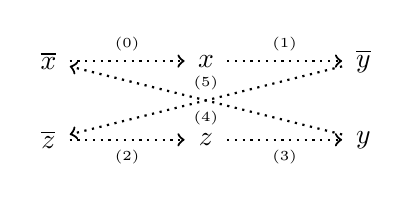
\begin{tikzpicture}
  \tikzset{vertex/.style = {draw=none,minimum size=1.5em,inner sep=0.5pt}}
  \tikzset{edge/.style = {-,-> = latex', dashed}}
  
  
\node[vertex] (ox)  at (0,1) {$\overline{x}$};
\node[vertex] (x)  at (2,1) {$x$};
\node[vertex] (y)  at (4,1) {$\overline{y}$};
\node[vertex] (oy)  at (4,0) {$y$};
\node[vertex] (z)  at (2,0) {$z$};
\node[vertex] (oz)  at (0,0) {$\overline{z}$};

  
    \path[->](ox) edge[dotted, thick] node [above]{\tiny(0)} (x);
      \path[->](x) edge[dotted, thick] node [above]{\tiny(1)} (y);
      
        \path[->](oz) edge[dotted, thick] node [below]{\tiny(2)} (z);
        \path[->](z) edge[dotted, thick] node [below]{\tiny(3)} (oy);
        
        \path[->](y) edge[dotted, thick] node [above]{\tiny(5)} (oz);
        \path[->](oy) edge[dotted, thick] node [below]{\tiny(4)} (ox);
   

\end{tikzpicture}
\end{center}
\end{itemize}
Having established that $\forall x\in \lit(\varphi) \; |\mathcal{J}(x)|\leq 1$, the second and third conditions follow directly from the construction of the algorithm. That is, as the algorithm always adds the complementary values to complementary literals, forcing  $\forall x \in \mathit{Lit}(\varphi)\;  \mathcal{J}(x) \cap \mathcal{J}(\overline{x}) = \emptyset$ under the knowledge that $\forall x\in \lit(\varphi) \; |\mathcal{J}(x)|\leq 1$ and as the truth values of a literal and its complement are assigned in immediate succession $|\mathcal{J}(x)| =| \mathcal{J}(\overline{x})|$ follows.
\end{itemize}
Finally, as \texttt{Step 1} consists of at most $|\lit(\varphi)|$ iterations of \texttt{Loop A}.\footnote{It is not intended for this bound to be tight.} The required statement is demonstrated.
\end{proof}

Using this one can move on towards the following Lemma.

\begin{lemma}
\label{lem:1-alt-step2}
Let $\varphi$ a 2-CNF formula. Suppose that there exists no variable $x \in \var(\varphi)$, s.t.\ both $x \sreach{\mathcal{G}(\varphi)} \ox$ and $\ox \sreach{\mathcal{G}(\varphi)}  x$ hold.
Let  $\mathcal{J}=\mathcal{A}(\varphi)$. Then it holds that for all literals $x$ in $\varphi$, $|\mathcal{J}(x)|\leq 1$ and $\mathcal{J}(x) \cap \mathcal{J}(\overline{x}) = \emptyset$ and $|\mathcal{J}(x)| =| \mathcal{J}(\overline{x})|$.
\end{lemma}
\begin{proof}
Again this result shall be demonstrated by means of induction. That is, under the assumption that $|\mathcal{J}(x)|\leq 1$ and $\mathcal{J}(x) \cap \mathcal{J}(\overline{x}) = \emptyset$ and $|\mathcal{J}(x)| =| \mathcal{J}(\overline{x})|$ after $n$ iterations of \texttt{Loop B}, it will be established that $|\mathcal{J}(x)|\leq 1$ and $\mathcal{J}(x) \cap \mathcal{J}(\overline{x}) = \emptyset$  and $|\mathcal{J}(x)| =| \mathcal{J}(\overline{x})|$ after $n+1$ iterations.

\begin{itemize}
\item \textbf{IH:} After $n$ iterations of \texttt{Loop B}, it holds that for all literals $x$ in $\varphi$, $|\mathcal{J}(x)|\leq 1$ and $\mathcal{J}(x) \cap \mathcal{J}(\overline{x}) = \emptyset \land |\mathcal{J}(x)| = |\mathcal{J}(\overline{x})|$.
\item \textbf{IB:} Clearly, before the first iteration Lemma \ref{lem:1-alt-step1} ensures that for all $x \in \lit(\varphi)$, $|\mathcal{J}(x)|\leq 1$ and $\mathcal{J}(x) \cap \mathcal{J}(\overline{x}) = \emptyset$ and $|\mathcal{J}(x)| =| \mathcal{J}(\overline{x})|$. Hence, the base case for $0$ iterations of \texttt{Loop B} is satisfied.

\item \textbf{IS:}  For the $n+1^{\text{th}}$ iteration to occur there must have been a $x \in \var(\varphi)$ such that $\mathcal{J}(x) =\mathcal{J}(\overline{x})= \emptyset$. Moreover, after said iteration it must be that for all $y \in \lit(\varphi)$ such that $x \reach y$ one has $\True \in \mathcal{J}(y)$. Assume there exists $y \in \lit(\varphi)$ such that $|\mathcal{J}(y)|=2$. 
\footnote{Again, before diving into the subsequent case distinction, notice that in the case $\mathcal{J}(y)=\{\}$ it could be that $y$ is $x$ or $\overline{x}$. Moreover, it is unnecessary to cover both of those possibilities, as (by construction) one can not exists without the other. That is, if $y=\overline{x}$ and $|\mathcal{J}(y)|=2$ after the  $n+1^{\text{th}}$ iteration, it must be by definition of $\mathcal{A}$ that  $|\mathcal{J}(x)|=2$ as well, thus allowing one to show this claim for $x$ only.  However, the subsequent cases are constructed such that they include those cases without explicitly engaging with them  (see the \emph{Appendix }for a demonstration of this claim). } 
Hence, there are three cases. 
\begin{itemize}
\item $\mathcal{J}(y)=\{\}$ before the $n+1^{\text{th}}$ iteration of \texttt{Loop B}. This is identical to the corresponding case in the proof of Lemma \ref{lem:1-alt-step1}. That is, it must be that $\True$ and $\False$  were added during the $n+1^{\text{th}}$ iteration of \texttt{Loop B}. This implies, by construction, that $x \reach y\; ^{(1)}$ and $x \reach \overline{y}\; ^{(2)}$. Using Lemma \ref{lem:inverse-path}, this implies that $y \reach \overline{x}\;^{(3)}$ and $\overline{y} \reach \overline{x}\;^{(4)}$. However, either is sufficient to establish that $x \reach \overline{x}$. Thereby, creating a cycle and subsequently a contradiction. 

\begin{center}
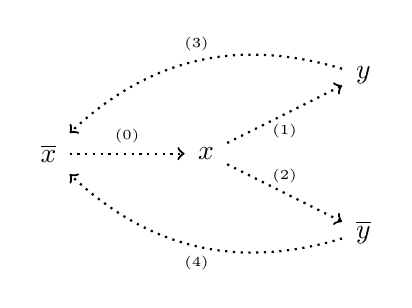
\begin{tikzpicture}
  \tikzset{vertex/.style = {draw=none,minimum size=1.5em,inner sep=0.5pt}}
  \tikzset{edge/.style = {-,-> = latex', dashed}}
  
  
\node[vertex] (ox)  at (0,1) {$\overline{x}$};
\node[vertex] (x)  at (2,1) {$x$};
\node[vertex] (y)  at (4,2) {$y$};
\node[vertex] (oy)  at (4,0) {$\overline{y}$};


  
    \path[->](ox) edge[dotted, thick] node [above]{\tiny(0)} (x);
      \path[->](x) edge[dotted, thick] node [below]{\tiny(1)} (y);
            \path[->](x) edge[dotted, thick, ] node [above]{\tiny(2)} (oy);
          
        
        \path[->](y) edge[dotted, thick, bend right=30] node [above]{\tiny(3)} (ox);
        \path[->](oy) edge[dotted, thick, bend left=30] node [below]{\tiny(4)} (ox);
   

\end{tikzpicture}
\end{center}


\item $\mathcal{J}(y)=\{\True\}$ before the iteration of \texttt{Loop B}. Then $\False$ must have been added during the iteration. However, this implies that $x \reach \overline{y}$. Now by Lemma \ref{lem:inverse-path}, it follows that $y \reach \overline{x}$. Now, if $\mathcal{J}(y)=\{\True\}$ then $\forall z \in \lit(\varphi)$ such that $y\reach z$ it must be the case that $\True \in \mathcal{J}(z)$. However, this includes $\overline{x}$ which by \textbf{IH} implies that $\False \in \mathcal{J}(x)$, contradicting the fact that $x$ was selected by the algorithm in the first place.
\item $\mathcal{J}(y)=\{\False\}$ before the iteration of \texttt{Loop B}. Then $\True$ must have been added during the iteration. However, this implies that $x \reach y$. Then from Lemma \ref{lem:inverse-path} it follows that $\overline{y} \reach \overline{x}$. By \textbf{IH}, it must be that 
$\mathcal{J}(\overline{y})=\{\True\}$ before the iteration. Since, it must be that $\forall z \in \lit(\varphi)$ such that $\overline{y} \reach z$ one has $\True \in \mathcal{J}(z)$, it follows from $\overline{y} \reach \overline{x}$ that $\True \in \mathcal{J}(\overline{x})$. Therefore, by \textbf{IH}, it must be the case that $\False \in \mathcal{J}(x)$, contradicting the fact that $x$ was selected by the algorithm in the first place.
\end{itemize}
Having established that $\forall x\in \lit(\varphi) \; |\mathcal{J}(x)|\leq 1$, the second and third conditions follow directly from the construction of the algorithm. That is, as the algorithm always adds the complementary values to complementary literals, forcing  $\forall x \in \mathit{Lit}(\varphi)\;  \mathcal{J}(x) \cap \mathcal{J}(\overline{x}) = \emptyset$ under the knowledge that $\forall x\in \lit(\varphi) \; |\mathcal{J}(x)|\leq 1$ and as the truth values of a literal and its complement are assigned in immediate succession $|\mathcal{J}(x)| =| \mathcal{J}(\overline{x})|$ follows.
%Having established that $\forall x\in \lit(\varphi) \; |\mathcal{J}(x)|\leq 1$, the second condition follows directly from the construction of the algorithm. That is, as the algorithm always adds the complementary values to complementary literals the second and third condition, $\forall x \in \mathit{Lit}(\varphi)\;  \mathcal{J}(x) \cap \mathcal{J}(\overline{x}) = \emptyset$ and $|\mathcal{J}(x)| =| \mathcal{J}(\overline{x})|$, follow immediately.
\end{itemize}
Finally, as \texttt{Step 2} consists of at most $|\var(\varphi)|$ iterations of \texttt{Loop B}.\footnote{Again, not a tight bound} The required statement is demonstrated.
\end{proof}


\begin{lemma}
\label{lem:1-alt}
Let $\varphi$ a 2-CNF formula. Let $\mathcal{J}:=\mathcal{A}(\varphi)$. Suppose that there exists no variable $x \in \var(\varphi)$, s.t.\ both $x \sreach{\mathcal{G}(\varphi)} \ox$ and $\ox \sreach{\mathcal{G}(\varphi)}  x$ hold.
%Then $\{ x \mathcal{J}|_{\var(\varphi)}$ is an appropriate truth assignment for $\varphi$. 
Then for all literals $x$ in $\varphi$ it holds that $|\mathcal{J}(x)|=1$ and $\mathcal{J}(x) \cap \mathcal{J}(\overline{x}) = \emptyset$.
\end{lemma}
\begin{proof}
This is a direct consequence of Lemma \ref{lem:1-alt-step2}. That is, from this lemma one obtains the assurance that $|\mathcal{J}(x)|\leq1$ and $\mathcal{J}(x) \cap \mathcal{J}(\overline{x}) = \emptyset$ and $|\mathcal{J}(x)| =| \mathcal{J}(\overline{x})|$ hold after \texttt{Step 2}, and thus implicitly after \texttt{Loop B}. However, this loop can only terminate, if there does not exists an $x \in \var(\varphi)$ such that $\mathcal{J}(x)=\emptyset$. Now given the fact that $\var(\varphi)$ is finite and that at every iteration one of the remaining undefined variables (and its complement) will be assigned at least one truth value, it must be that \texttt{Loop B} terminates. Hence, ensuring that $|\mathcal{J}(x)|=1$ holds.
\end{proof}

\begin{remark}
The reason why there does not exists an $x$ such that $\mathcal{J}(x)=\emptyset$ is essentially the reason why $\mathcal{I}$, is actually an \emph{appropriate} truth assignment for $\varphi$.
\end{remark}
It is clear that the following Lemma is equivalent to Lemma \ref{lem:1}. However, to be sure consider the following.

\begin{lemma}
\label{lem:connect}
Lemma \ref{lem:1} is implied by Lemma \ref{lem:1-alt}.
\end{lemma}
\begin{proof}
To demonstrate the claim, it is sufficient to establish that 
if for all literals $x$ in $\varphi$ it holds that $|\mathcal{J}(x)|=1$ and $\mathcal{J}(x) \cap \mathcal{J}(\overline{x}) = \emptyset$, then the truth assigment $\mathcal{I}$ constructed by $\mathcal{A}$ is never changed later.
% then it follows that it cannot happen, that at some stage, 
%$\II (z) =\True$ for some variable $z$ and later this value is changed to 
%$\II (z) =\False$ or vice versa.
To that end, assume that for all literals $x$ in $\varphi$ it holds that $|\mathcal{J}(x)|=1$ and $\mathcal{J}(x) \cap \mathcal{J}(\overline{x}) = \emptyset$ and $|\mathcal{J}(x)| =| \mathcal{J}(\overline{x})|$. And assume that there exists a $x \in \var(\varphi)$ such that the truth value $\mathcal{I}(x)$ was changed during the construction of $\mathcal{I}$ in $\mathcal{A}$. 
Assume that $\mathcal{I}(x)=\True$ was changed to $\mathcal{I}(x)=\False$. This implies that first the line "$\mathcal{I}(x):=\True$" and later the line "$\mathcal{I}(\overline{x}):=\True$" had to be executed at one point in the algorithm. However, by definition of $\mathcal{A}$ this is only possible, if initially "$\mathcal{J}(x):=\mathcal{J}(x) \cup \True$" and "$\mathcal{I}(\overline{x}):=\mathcal{J}(\overline{x}) \cup \False$" and then "$\mathcal{J}(\overline{x}):=\mathcal{J}(\overline{x}) \cup \True$" and "$\mathcal{I}(x):=\mathcal{J}(x) \cup \False$" were executed. However, this would imply that there exists an $x$ such that $|\mathcal{J}(x)|=2$, which is clearly a contradiction.

The other case is merely an analogue to the previous one.\footnote{That is, assume that $\mathcal{I}(x)=\False$ was changed to $\mathcal{I}(x)=\True$. This implies that first the line "$\mathcal{I}(\overline{x}):=\True$" and later the line "$\mathcal{I}(x):=\True$" had to be executed at one point in the algorithm. However, by definition of $\mathcal{A}$ this is only possible, if initially "$\mathcal{J}(\overline{x}):=\mathcal{J}(\overline{x}) \cup \True$" and "$\mathcal{I}(x):=\mathcal{J}(x) \cup \False$" and then "$\mathcal{J}(x):=\mathcal{J}(x) \cup \True$" and "$\mathcal{I}(\overline{x}):=\mathcal{J}(\overline{x}) \cup \False$" were executed. However, this is clearly a contradiction.}
 Therefore, it is ensured that if for all literals $x$ in $\varphi$ it holds that $|\mathcal{J}(x)|=1$ and $\mathcal{J}(x) \cap \mathcal{J}(\overline{x}) = \emptyset$, no reassignment occurred during the construction of $\mathcal{I}$.
\end{proof}

%
%Moreover, the following can be observed.
%
%\begin{lemma}
%\label{lem:equal}
%Let $\varphi$ a 2-CNF formula. Let $\mathcal{J}:=\mathcal{A}(\varphi)$. Suppose that there exists no variable $x \in \var(\varphi)$, s.t.\ both $x \sreach{\mathcal{G}(\varphi)} \ox$ and $\ox \sreach{\mathcal{G}(\varphi)}  x$ hold.
%%Then $\{ x \mathcal{J}|_{\var(\varphi)}$ is an appropriate truth assignment for $\varphi$. 
%Then $\mathcal{I}$ as constructed during $\mathcal{A}$, is equal to $\mathcal{I}_{\mathcal{J}}\{ x\mapsto y \mid \forall x\in \var(\varphi) \; y \in \mathcal{J}(x)\}$.
%\end{lemma}
%\begin{proof}
%By Lemma \ref{lem:1-alt}, it is ensured that $\forall x\in \var(\varphi) \; |\mathcal{J}(x)|$, making $\mathcal{I}_{\mathcal{J}}$ well defined. Through this assurance in a slight abuse of notation let $\mathcal{J}(x)=\{ y\}$ for $y \in \{\True, \False\}$ be read as $\mathcal{J}(x)=y$.
%Assume that there exists a variable $x\in \var(\varphi)$ such that $\mathcal{I}(x)\neq \mathcal{J}(x)$. It was established through  Lemma \ref{lem:connect} that no reassignment happens. Now by construction, for any $x\in \var(\varphi)$, $\mathcal{I}$ and $\mathcal{J}$ are constructed such that $x$ obtains the same truth value (negative values are assigned explicitly in $\mathcal{J}$, while only implicitly in $\mathcal{I}$) this is an impossibility.  
%\end{proof}
%\begin{definition}
%Let $\varphi$ a 2-CNF formula. Then  we definite $\mathcal{J}_{\varphi}$ as a the function $\mathcal{J}_{\varphi}: \mathcal{G}(\varphi) \to \mathcal{P}(\{ 0,1\})\setminus \emptyset$ such that for $v \in V(\mathcal{G}(\varphi))$, $\mathcal{J}_{\varphi}(v)= \mathcal{J}_{\varphi}^2\big(\mathcal{J}_{\varphi}^1(v),v\big)$. \footnote{$\mathcal{P}(X)$ denotes the powerset of $X$.} Furthermore, $\mathcal{J}_{\varphi}^1: \mathcal{G}(\varphi) \to \mathcal{P}(\{ 0,1\})\setminus \emptyset$ is recursively defined 
%\begin{itemize}
%\item 
%\end{itemize}
%$v \in V(\mathcal{G}(\varphi))$ $\mathcal{J}_{\varphi}^1(v)=$
%\end{definition}





\newpage

  
\noindent

\begin{exercise}[2 credits]
{\em Give a rigorous proof of Lemma \ref{lem:2}.
}%em
\end{exercise}


\noindent
\paragraph*{Solution}


Lemma \ref{lem:2} can be proven directly.

\begin{proof}(Lemma \ref{lem:2})
Let $\varphi$ a 2-CNF formula where there exists no variable $x \in \var(\varphi)$, s.t.\ both $x \sreach{\mathcal{G}(\varphi)} \ox$ and $\ox \sreach{\mathcal{G}(\varphi)}  x$ hold.
Assume that interpretation $\mathcal{I}$, as constructed by $\mathcal{A}(\varphi)$, does not satisfy $\varphi$. Hence, there must exist a clause $(x \lor y) \in \clau(\varphi)$ such that $\mathcal{I}(x)=\mathcal{I}(y)=\False$.
By construction of $\mathcal{G}(\varphi)$ it is known $(\alpha , \beta) \in E(\mathcal{G}(\varphi))$ iff $(\overline{\alpha} \lor \beta)\in  \clau(\varphi)$ or $(\beta \lor \overline{\alpha})\in  \clau(\varphi)$. Therefore, it must be that 
$(\overline{x}, y) \in E(\mathcal{G}(\varphi))$ and $(\overline{y}, x) \in E(\mathcal{G}(\varphi))$. By definition of $\mathcal{A}$, if some literal was assigned the value $\True$ all reachable literals must also be assigned the value $\True$. It is known that $\mathcal{I}(x)=\mathcal{I}(y)=\False$. Hence, by semantics $\mathcal{I}(\overline{x})=\mathcal{I}(\overline{y})=\True$. W.l.o.g assume that $x$ was assigned its truth value first. Therefore, after the step where $x$ was given its truth value,  it must be that $\forall z \in \lit(\varphi)\; \overline{x} \reach z$ one has $\mathcal{I}(z) = \True$. However, as $(\overline{x}, y) \in E(\mathcal{G}(\varphi))$ it follows that $\mathcal{I}(y)=\True$. By assumption it is known that $\mathcal{I}(y)=\False$. Hence, the truth value of $y$ must have undergone a reassignment, which clearly is a contradiction.

%\begin{center}
%\begin{tikzpicture}
%  \tikzset{vertex/.style = {draw=none,minimum size=1.5em,inner sep=0.5pt}}
%  \tikzset{edge/.style = {-,-> = latex', dashed}}
%  
%  
%\node[vertex] (ox)  at (0,1) {$\overline{x}$};
%\node[vertex] (x)  at (2,0) {$x$};
%\node[vertex] (y)  at (2,1) {$y$};
%\node[vertex] (oy)  at (0,0) {$\overline{y}$};
%
%
%  
%    \path[->](ox) edge node [above]{} (y);
%      \path[->](oy) edge node [above]{} (x);
%   
%   
%
%\end{tikzpicture}
%\end{center}


\end{proof}

\newpage
\paragraph*{Appendix}



The only aim is to demonstrate that the cases $y=x$ and $y = \overline{x}$ are actually covered by the cases in the main part of the proof. To do so, they barely edited, meaning that even if the claim was already demonstrated the proof remains identical in structure as the cases in the main part of the proof. That is their sole purpose. \emph{Hence, the arguments are absolutely \textbf{ridiculous} to read.}

\bigskip
Here the additional information for the proof of Lemma \ref{lem:1-alt-step1}. Firstly, in the case of $y=x$.
\begin{itemize}
\item $\mathcal{J}(x)=\{\}$ before the $n+1^{\text{th}}$ iteration of \texttt{Loop A}. Hence, it must be that $\True$ and $\False$  must have been added during the $n+1^{\text{th}}$ iteration of \texttt{Loop A}. This implies, by construction, that $x \reach x\; ^{(1)}$ and $x \reach \overline{x}\; ^{(2)}$. Using Lemma \ref{lem:inverse-path}, this implies that $x \reach \overline{x}\;^{(3)}$ and $\overline{x} \reach \overline{x}\;^{(4)}$. However, only one of those is sufficient to establish that $x \reach \overline{x}$. Thereby, creating a cycle and subsequently a contradiction. 

\begin{center}
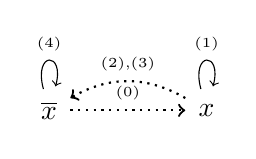
\begin{tikzpicture}
  \tikzset{vertex/.style = {draw=none,minimum size=1.5em,inner sep=0.5pt}}
  \tikzset{edge/.style = {-,-> = latex', dashed}}
  
  
\node[vertex] (ox)  at (0,1) {$\overline{x}$};
\node[vertex] (x)  at (2,1) {$x$};
%\node[vertex] (y)  at (4,2) {$x$};
%\node[vertex] (oy)  at (4,0) {$\overline{x}$};


  
    \path[->](ox) edge[dotted, thick] node [above]{\tiny(0)} (x);
    	\draw (x) edge[loop above] node{\tiny(1)} (x);
%      \path[->](x) edge[dotted, thick] node [below]{\tiny(1)} (y);
%            \path[->](x) edge[dotted, thick, ] node [above]{\tiny(2)} (ox);
          
        
        \path[->](x) edge[dotted, thick, bend right=30] node [above]{\tiny(2),(3)} (ox);
        \draw (ox) edge[loop above] node{\tiny(4)} (ox);
%        \path[->](ox) edge[dotted, thick, bend left=30] node [below]{\tiny(4)} (ox);
   

\end{tikzpicture}
\end{center}
 
 
 
\item $\mathcal{J}(x)=\{\False\}$ before the $n+1^{\text{th}}$ iteration of \texttt{Loop A}. Therefore, $\True$ must have been added. Hence, it must be that $x \reach x\;^{(1)}$, as otherwise $\True$ would not have been added in the $n+1^{\text{th}}$ iteration of \texttt{Loop A}. Moreover, by \textbf{IH} it must be that $\mathcal{J}(\overline{x})=\{\True\}$ before the $n+1^{\text{th}}$ iteration of \texttt{Loop A}. This implies, by definition of \texttt{Loop A}, that there must exist a $z \in \lit(\varphi)$ such that 
$\overline{z} \reach z\; ^{(2)}$ and $z \reach \overline{x}\; ^{(3)}$. Now, from $z \reach \overline{x}$ one obtains $x \reach \overline{z}\;^{(4)}$ 
through Lemma \ref{lem:inverse-path}. Similarly, one obtains from $x \reach x$ that $\overline{x} \reach \overline{x}\;^{(5)}$. Thereby, creating a cycle and thus a contradiction.

\begin{center}
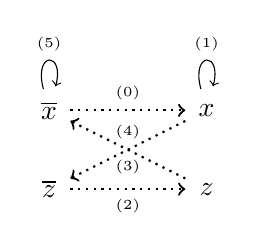
\begin{tikzpicture}
  \tikzset{vertex/.style = {draw=none,minimum size=1.5em,inner sep=0.5pt}}
  \tikzset{edge/.style = {-,-> = latex', dashed}}
  
  
\node[vertex] (ox)  at (0,1) {$\overline{x}$};
\node[vertex] (x)  at (2,1) {$x$};
%\node[vertex] (y)  at (4,1) {$y$};
%\node[vertex] (oy)  at (4,0) {$\overline{y}$};
\node[vertex] (z)  at (2,0) {$z$};
\node[vertex] (oz)  at (0,0) {$\overline{z}$};

  
    \path[->](ox) edge[dotted, thick] node [above]{\tiny(0)} (x);
   	\draw (x) edge[loop above] node{\tiny(1)} (x);
      
        \path[->](oz) edge[dotted, thick] node [below]{\tiny(2)} (z);
        \path[->](z) edge[dotted, thick] node [below]{\tiny(3)} (ox);
        
        \path[->](x) edge[dotted, thick] node [above]{\tiny(4)} (oz);
         	\draw (ox) edge[loop above] node{\tiny(5)} (ox);
%       \path[->](ox) edge[dotted, thick] node [below]{\tiny(4)} (ox);
   

\end{tikzpicture}
\end{center}
 

\item $\mathcal{J}(x)=\{\True\}$ before the $n+1^{\text{th}}$ iteration of \texttt{Loop A}. Thus, by \textbf{IH} it must be that $\mathcal{J}(\overline{x})=\{\False\}$ before the said iteration. If $\False$ was added to $\mathcal{J}(x)$ at the $n+1^{\text{th}}$ iteration, then by construction it must be that $\True$ was added to $\mathcal{J}(\overline{x})$ at the same time. However, for $\True$ to be added to a literal at step $n+1$ if must be that it is reachable from $x$. Hence, one obtains that $x \reach \overline{x}\;^{(1)}$. 
%As a side note, observe that this covers the case where $y=\overline{x}$ and that the case $y=x$ is an impossibility.
Now the argument is an analogue to the previous case. That is, as $\mathcal{J}(x)=\{\True\}$ after iteration $n$. Again by definition of \texttt{Loop A}  it must be the case that there exist a $z\in \lit(\varphi)$ such that $\overline{z} \reach z\;^{(2)}$ and $z \reach x\;^{(3)}$. Now from Lemma \ref{lem:inverse-path}, one obtains $x \reach \overline{x}\;^{(4)}$ from $x \reach \overline{x}$ and  $\overline{x} \reach \overline{z}\;^{(5)}$ from $z \reach x$. Thereby, creating a cycle and thus a contradiction.

\begin{center}
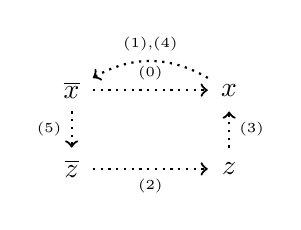
\begin{tikzpicture}
  \tikzset{vertex/.style = {draw=none,minimum size=1.5em,inner sep=0.5pt}}
  \tikzset{edge/.style = {-,-> = latex', dashed}}
  
  
\node[vertex] (ox)  at (0,1) {$\overline{x}$};
\node[vertex] (x)  at (2,1) {$x$};
%\node[vertex] (y)  at (4,1) {$\overline{y}$};
%\node[vertex] (oy)  at (4,0) {$y$};
\node[vertex] (z)  at (2,0) {$z$};
\node[vertex] (oz)  at (0,0) {$\overline{z}$};

  
    \path[->](ox) edge[dotted, thick] node [above]{\tiny(0)} (x);
      \path[->](x) edge[dotted, thick, bend right=30] node [above]{\tiny(1),(4)} (ox);
%      \path[->](x) edge[dotted, thick] node [above]{\tiny(1)} (y);
      
        \path[->](oz) edge[dotted, thick] node [below]{\tiny(2)} (z);
        \path[->](z) edge[dotted, thick] node [right]{\tiny(3)} (x);
        
        \path[->](ox) edge[dotted, thick] node [left]{\tiny(5)} (oz);
%         	\draw (ox) edge[loop above] node{\tiny(4)} (ox);
%        \path[->](ox) edge[dotted, thick] node [below]{\tiny(4)} (ox);
   

\end{tikzpicture}
\end{center}
\end{itemize}
\noindent
Secondly, in the case of $y=\overline{x}$. Meaning that $|\mathcal{J}(\overline{x})|=2$ after $n+1$ iterations of \texttt{Loop A}. However, by definition of $\mathcal{A}$ and by the \textbf{IH}, it must be that $|\mathcal{J}(x)|=2$ after $n+1$ iterations of \texttt{Loop A}.
Hence, w.l.o.g. it is possible to show the claim for $x$, which was already done. Thereby, closing this case as well.

\bigskip

Similarly, for the proof in Lemma \ref{lem:1-alt-step2}, in the case of $y=x$ consider the following.


\begin{itemize}
\item $\mathcal{J}(x)=\{\}$ before the $n+1^{\text{th}}$ iteration of \texttt{Loop B}. Hence, it must be that $\True$ and $\False$  must have been added during the $n+1^{\text{th}}$ iteration of \texttt{Loop B}. This implies, by construction, that $x \reach x\; ^{(1)}$ and $x \reach \overline{x}\; ^{(2)}$. Using Lemma \ref{lem:inverse-path}, this implies that $x \reach \overline{x}\;^{(3)}$ and $\overline{x} \reach \overline{x}\;^{(4)}$. However, only one of those is sufficient to establish that $x \reach \overline{x}$. Thereby, creating a cycle and subsequently a contradiction. 

\begin{center}
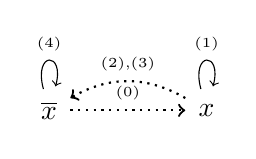
\begin{tikzpicture}
  \tikzset{vertex/.style = {draw=none,minimum size=1.5em,inner sep=0.5pt}}
  \tikzset{edge/.style = {-,-> = latex', dashed}}
  
  
\node[vertex] (ox)  at (0,1) {$\overline{x}$};
\node[vertex] (x)  at (2,1) {$x$};
%\node[vertex] (y)  at (4,2) {$x$};
%\node[vertex] (oy)  at (4,0) {$\overline{x}$};


  
    \path[->](ox) edge[dotted, thick] node [above]{\tiny(0)} (x);
    	\draw (x) edge[loop above] node{\tiny(1)} (x);
%      \path[->](x) edge[dotted, thick] node [below]{\tiny(1)} (y);
%            \path[->](x) edge[dotted, thick, ] node [above]{\tiny(2)} (ox);
          
        
        \path[->](x) edge[dotted, thick, bend right=30] node [above]{\tiny(2),(3)} (ox);
        \draw (ox) edge[loop above] node{\tiny(4)} (ox);
%        \path[->](ox) edge[dotted, thick, bend left=30] node [below]{\tiny(4)} (ox);
   

\end{tikzpicture}
\end{center}
 
 \end{itemize}
Notice that the cases $\mathcal{J}(x)=\{\True\}$ and  $\mathcal{J}(x)=\{\False\}$ are, by definition of \texttt{Loop B} an impossibility. 

%
%The other cases are an impossibility. However, for the sake of completion consider the following.
%
%\begin{itemize}
%\item $\mathcal{J}(x)=\{\True\}$ before the iteration of \texttt{Loop B}. Then $\False$ must have been added during the iteration. However, this implies that $x \reach \overline{x}$. Now by Lemma \ref{lem:inverse-path}, it follows that $x \reach \overline{x}$. Now, if $\mathcal{J}(x)=\{\True\}$ then $\forall z \in \lit(\varphi)$ such that $x\reach z$ it must be the case that $\True \in \mathcal{J}(z)$. However, this includes $\overline{x}$. 
%By \textbf{IH}, it must therefore be the case that $\False \in \mathcal{J}(x)$, contradicting the fact that $x$ was selected by the algorithm in the first place.
%\item $\mathcal{J}(x)=\{\False\}$ before the iteration of \texttt{Loop B}. Then $\True$ must have been added during the iteration. However, this implies that $x \reach x$. Then from Lemma \ref{lem:inverse-path} it follows that $\overline{x} \reach \overline{x}$. By \textbf{IH}, it must be that 
%$\mathcal{J}(\overline{x})=\{\True\}$ before the iteration. Hence, it must be that $\forall z \in \lit(\varphi)$ such that $\overline{x} \reach z$ one has $\True \in \mathcal{J}(z)$. Hence, from $\overline{x} \reach \overline{x}$ it follows that $\True \in \mathcal{J}(\overline{x})$. Therefore, by \textbf{IH}, it must therefore be the case that $\False \in \mathcal{J}(x)$, contradicting the fact that $x$ was selected by the algorithm in the first place.
%\end{itemize}

As for the case $y=\overline{x}$. The same argument as in addendum of Lemma \ref{lem:1-alt-step1} can be applied.

\end{document}


